\section{Dockerizar su aplicación}

\subsection{Uso de Dockerfile y Docker Compose}
Cada servicio tiene su propio \texttt{Dockerfile} en su carpeta (\texttt{backend/}, \texttt{frontend/}) y un \texttt{.dockerignore} que excluye \texttt{.venv}, \texttt{node\_modules} y archivos de entorno. El archivo \texttt{docker/docker-compose.yaml} orquesta los tres servicios:

\begin{itemize}
    \item \textbf{postgres}: imagen oficial \texttt{postgres:16.3}, contraseña inyectada como \emph{secret} de Compose (\texttt{POSTGRES\_PASSWORD\_FILE}) en lugar de variable de entorno en claro, volumen nombrado para persistir datos y \emph{healthcheck} con \texttt{pg\_isready}.
    \item \textbf{backend}: se construye desde \texttt{backend/Dockerfile}, lee \texttt{SECRET\_KEY} y \texttt{POSTGRES\_PASSWORD} de \texttt{.env.dev} (ignorado por Git), y declara \texttt{depends\_on: postgres: condition: service\_healthy}, de modo que uvicorn arranca solo cuando la base acepta conexiones.
    \item \textbf{frontend}: se construye desde \texttt{frontend/Dockerfile} y depende del backend.
\end{itemize}

Hay dos redes: \texttt{public}, a la que se conectan frontend y backend para exponer los puertos 3000 y 8000 al host, y \texttt{private} con \texttt{internal: true}, la única a la que pertenece Postgres, que por tanto no es alcanzable desde fuera del stack.

El \texttt{Dockerfile} del backend aplica las mejores prácticas de seguridad y eficiencia: usa un patrón de dos pasos con \texttt{uv} para aprovechar la caché de capas (instalando primero dependencias), copia explícitamente solo el código fuente necesario en lugar de un \texttt{COPY . .} indiscriminado, configura un usuario \emph{non-root} (\texttt{appuser}), y levanta la aplicación con el comando oficial para producción \texttt{fastapi run}.

\begin{lstlisting}[language=bash,caption={backend/Dockerfile}]
FROM python:3.13-slim

# Install uv
COPY --from=ghcr.io/astral-sh/uv:latest /uv /uvx /bin/

# Create a non-root user
RUN groupadd -r appuser && useradd -r -g appuser appuser

WORKDIR /app

# Copy dependency files and install dependencies
COPY pyproject.toml uv.lock ./
RUN uv sync --frozen --no-dev --no-install-project

# Copy only the necessary application source code directories
COPY api api/
COPY core core/
COPY models models/
COPY schemas schemas/
COPY main.py .

# Install the project itself (without dev dependencies)
RUN uv sync --frozen --no-dev

# Set permissions for the non-root user
RUN chown -R appuser:appuser /app
USER appuser

# Put the virtual environment in the PATH
ENV PATH="/app/.venv/bin:$PATH"

EXPOSE 8000

# Start FastAPI application using the production CLI
CMD ["fastapi", "run", "main.py", "--host", "0.0.0.0", "--port", "8000"]
\end{lstlisting}

Para el \texttt{Dockerfile} del frontend se implementa un patrón de compilación multi-etapa (\emph{multi-stage build}). La etapa \texttt{builder} compila la aplicación, pero la etapa final \texttt{runner} solo hereda el servidor independiente \emph{standalone} ultraligero que genera Next.js, descartando todo el código fuente original y dependencias de desarrollo para mayor seguridad y menor tamaño de imagen. Adicionalmente, el servicio se ejecuta bajo un usuario sin privilegios (\texttt{nextjs}).

\begin{lstlisting}[language=bash,caption={frontend/Dockerfile}]
FROM node:20-alpine AS base
RUN corepack enable && corepack prepare pnpm@9.6.0 --activate

# 1. Dependencies stage
FROM base AS deps
WORKDIR /app
COPY package.json pnpm-lock.yaml ./
RUN pnpm install --frozen-lockfile

# 2. Build stage
FROM base AS builder
WORKDIR /app
COPY --from=deps /app/node_modules ./node_modules
COPY . .
RUN pnpm run build

# 3. Production runner stage
FROM base AS runner
WORKDIR /app
ENV NODE_ENV=production

# Create non-root user
RUN addgroup -g 1001 -S nodejs && adduser -S nextjs -u 1001

# Copy only the necessary files from builder
COPY --from=builder /app/public ./public
COPY --from=builder --chown=nextjs:nodejs /app/.next/standalone ./
COPY --from=builder --chown=nextjs:nodejs /app/.next/static ./.next/static

USER nextjs

EXPOSE 3000
ENV PORT=3000
ENV HOSTNAME="0.0.0.0"

CMD ["node", "server.js"]
\end{lstlisting}

\subsection{Ejemplo del servicio web y base de datos}
Fragmento de \texttt{docker/docker-compose.yaml} con el servicio web (backend FastAPI) y la base de datos:

\begin{lstlisting}[caption={docker/docker-compose.yaml (extracto)}]
services:
  backend:
    build: { context: ../backend, dockerfile: Dockerfile }
    ports: ["8000:8000"]
    env_file: [.env.dev]          # SECRET_KEY, POSTGRES_PASSWORD
    environment:
      - POSTGRES_SERVER=postgres
      - POSTGRES_DB=mydb
      - POSTGRES_USER=myuser
    networks: [public, private]
    depends_on:
      postgres:
        condition: service_healthy

  postgres:
    image: postgres:16.3
    restart: always
    environment:
      - POSTGRES_USER=myuser
      - POSTGRES_DB=mydb
      - POSTGRES_PASSWORD_FILE=/run/secrets/pg_password
    secrets: [pg_password]
    volumes: [postgres-data:/var/lib/postgresql/data]
    networks: [private]
    healthcheck:
      test: ["CMD-SHELL", "pg_isready -U myuser -d mydb"]
      interval: 5s
      timeout: 5s
      retries: 5

secrets:
  pg_password: { file: ./pg_password.txt }
volumes:
  postgres-data:
networks:
  public:
  private: { internal: true }
\end{lstlisting}

Para levantar el stack basta con crear los dos archivos de secretos (no versionados) y ejecutar Compose desde \texttt{docker/}:

\begin{lstlisting}[language=bash]
$ cd docker
$ printf 'POSTGRES_PASSWORD=devops123\nSECRET_KEY=replace-me-with-at-least-32-random-characters\n' > .env.dev
$ echo devops123 > pg_password.txt
$ docker compose -p misiops up --build -d
\end{lstlisting}

\subsection{Evidencia que su aplicación está corriendo en docker}
El Listado~\ref{lst:dockerps} muestra los tres contenedores en ejecución el 21 de septiembre de 2026 y la respuesta de cada servicio desde el host. El workflow \texttt{docker-integration.yml} levanta el stack y verifica el backend en cada PR; la comprobación del frontend mostrada en este listado corresponde a la ejecución local.

\begin{lstlisting}[caption={\texttt{docker compose ps} y comprobación de los servicios},label={lst:dockerps}]
$ docker compose -p misiops ps
NAME                 IMAGE              STATUS                    PORTS
misiops-backend-1    misiops-backend    Up 32 seconds             0.0.0.0:8000->8000/tcp
misiops-frontend-1   misiops-frontend   Up 32 seconds             0.0.0.0:3000->3000/tcp
misiops-postgres-1   postgres:16.3      Up 37 seconds (healthy)   5432/tcp

$ curl http://localhost:8000/
{"status":"ok"}

$ curl -o /dev/null -w '%{http_code}\n' http://localhost:3000/
200
\end{lstlisting}

\begin{figure}[H]
    \centering
    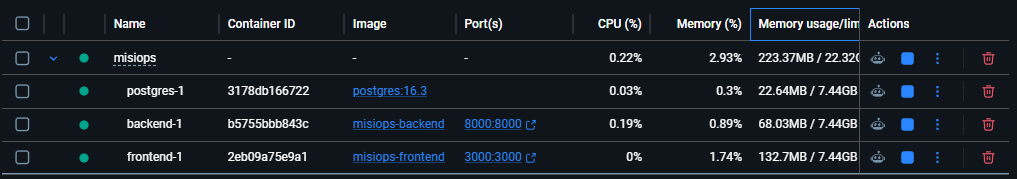
\includegraphics[width=0.95\textwidth]{figures/docker/docker-desktop.png}
    \caption{Los tres contenedores del proyecto \texttt{misiops} en ejecución en Docker Desktop, con los puertos 8000 y 3000 publicados y Postgres sin puerto expuesto}
    \label{fig:docker_running}
\end{figure}

La Figura~\ref{fig:docker_app} muestra la aplicación servida por el contenedor \texttt{frontend} en el puerto 3000 (atendido por el proxy de Docker, sin ningún servidor de desarrollo local), con una sesión iniciada. Los montos del tablero los calcula el endpoint \texttt{/api/v1/transactions/summary} del contenedor \texttt{backend} a partir de los datos persistidos en el contenedor \texttt{postgres}, de modo que la captura ejercita los tres servicios a la vez.

\begin{figure}[H]
    \centering
    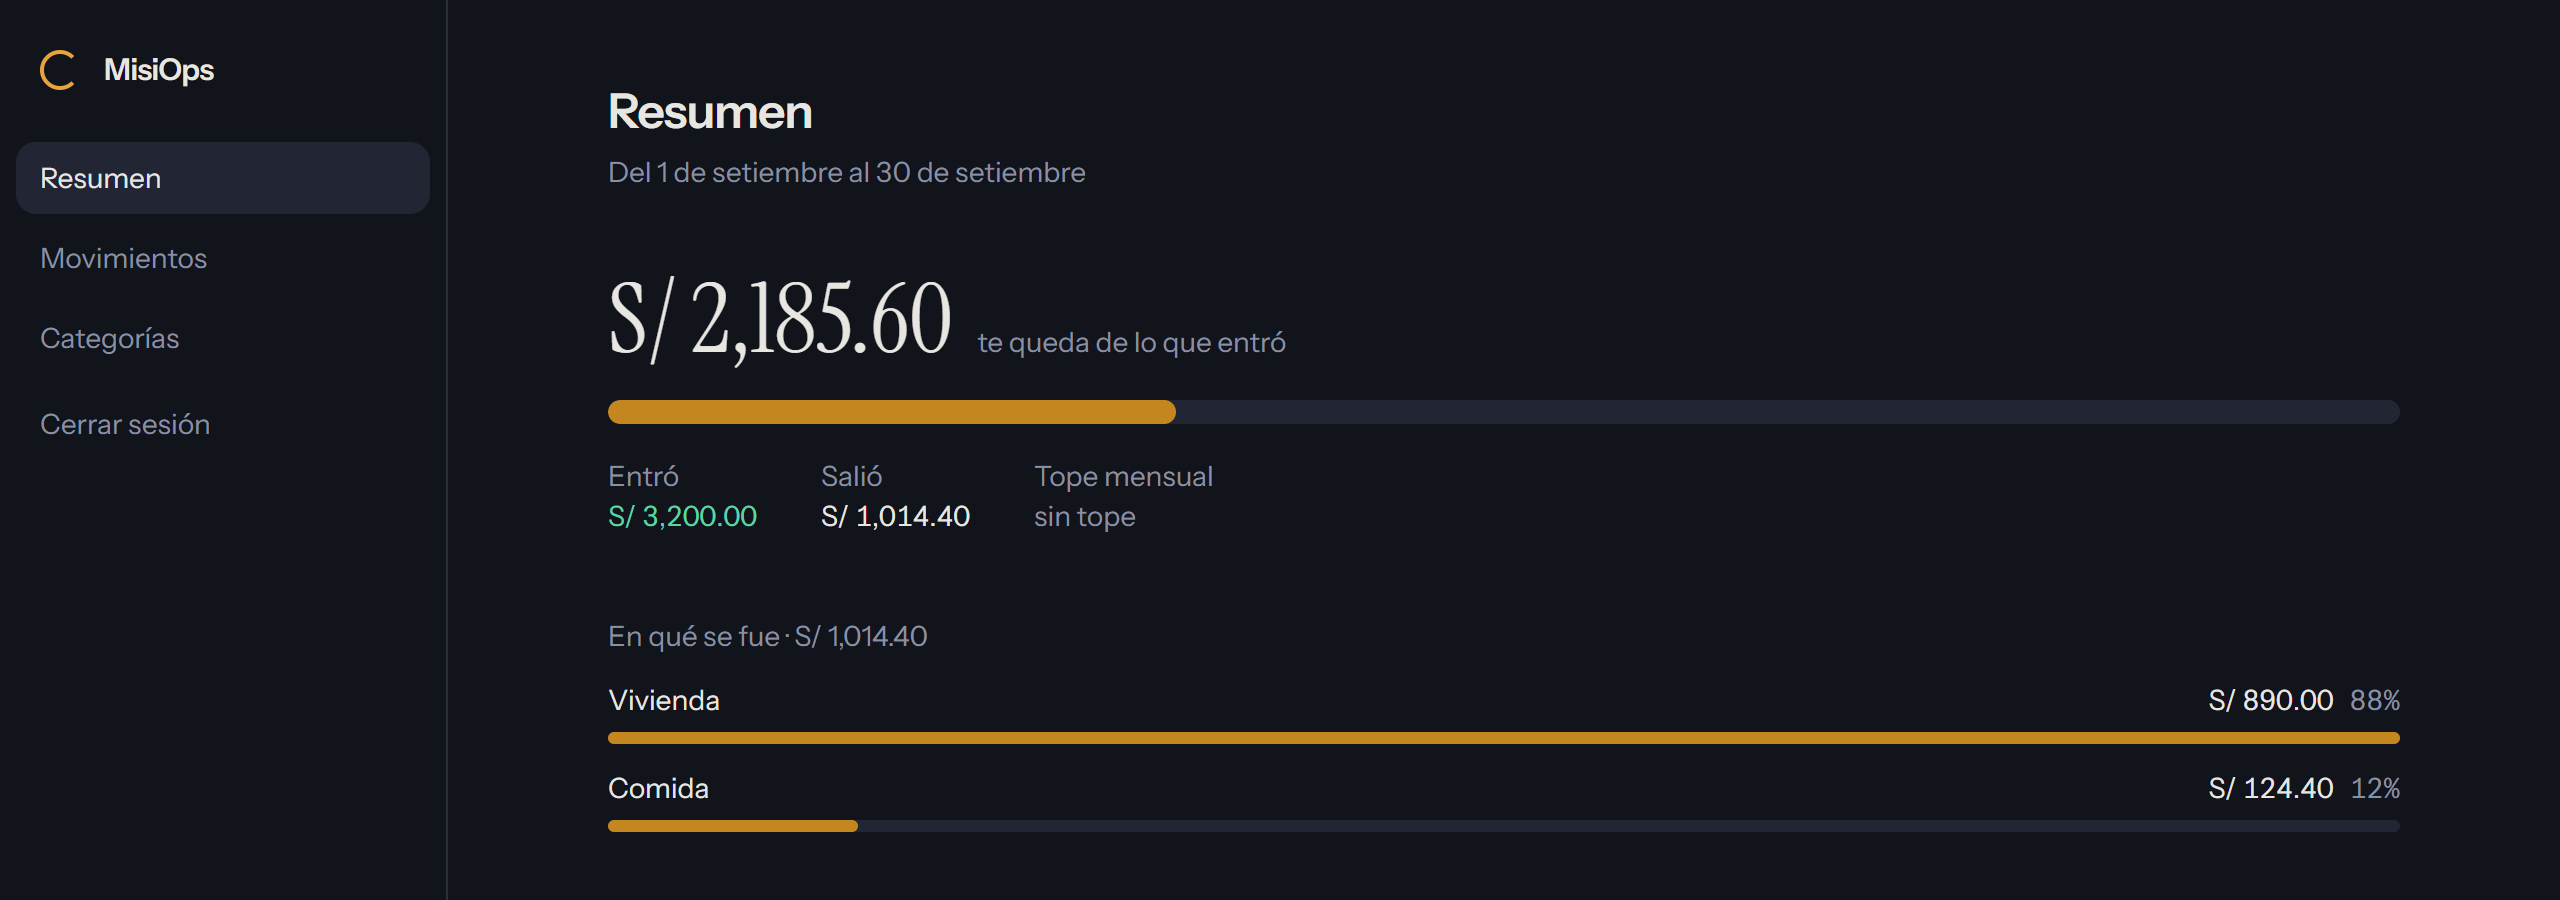
\includegraphics[width=0.95\textwidth]{figures/docker/docker-app.png}
    \caption{Tablero de MisiOps servido desde Docker en \texttt{http://localhost:3000}, con datos reales de la base de datos}
    \label{fig:docker_app}
\end{figure}
